\subsection{Dataset Combined and Feature Importance Identified}
% Summarize findings from the data quality checks and feature importance analyses.
The first result from our investigation is a combined dataset, aligned and harmonized as shown in Supplementary Material Table S2. Upon these alignment, we examined the percentage of fill on each of these columns, and ended up dropping columns that are not filled up to 50\%. This gave us a relatively clean dataset that we then proceeded to examine relevant features that can be selected via AutoML (\texttt{Pycaret}) after generating relevant features through geographical tools (\texttt{geopy}) and analytical-model-backed \texttt{pythermalcomfort}.

% methodology and model setup
We ended up selecting 20 features out of the 51 features (including physiological-model-derived $T_{core}$, $T_{skin}$, and $w$ from both Gagge and JOS-3 models) by selecting the top features with the help of AutoML. After adequate preprocessing and normalizing with MinMaxScaler, we set up an experiment in \texttt{Pycaret} to perform regression on the \textit{thermal sensation} column. Through comparison of the performance across 17 different regression models, Random Forrest and LightGBM are selected as the two top performers. As we care a lot about the solution not overfitting, we opted for LightGBM to identify the top features. The fitted LightGBM regressor with 10 folds is shown in Figure~\ref{fig:lgb-featimp} to illustrate their Shapley values in terms of their contributions towards the $TSV$ prediction. Shapley values originated from a solution concept in game theory when two or more players or factors are involved in a strategy to achieve a desired outcome or payoff, which later became a widely-used tool to evaluate predictive power of input features in aggregate. Here in Figure~\ref{fig:lgb-featimp}, every point represents the level of contribution from the current feature to its corresponding target.

\begin{figure}[h!]
    \centering
    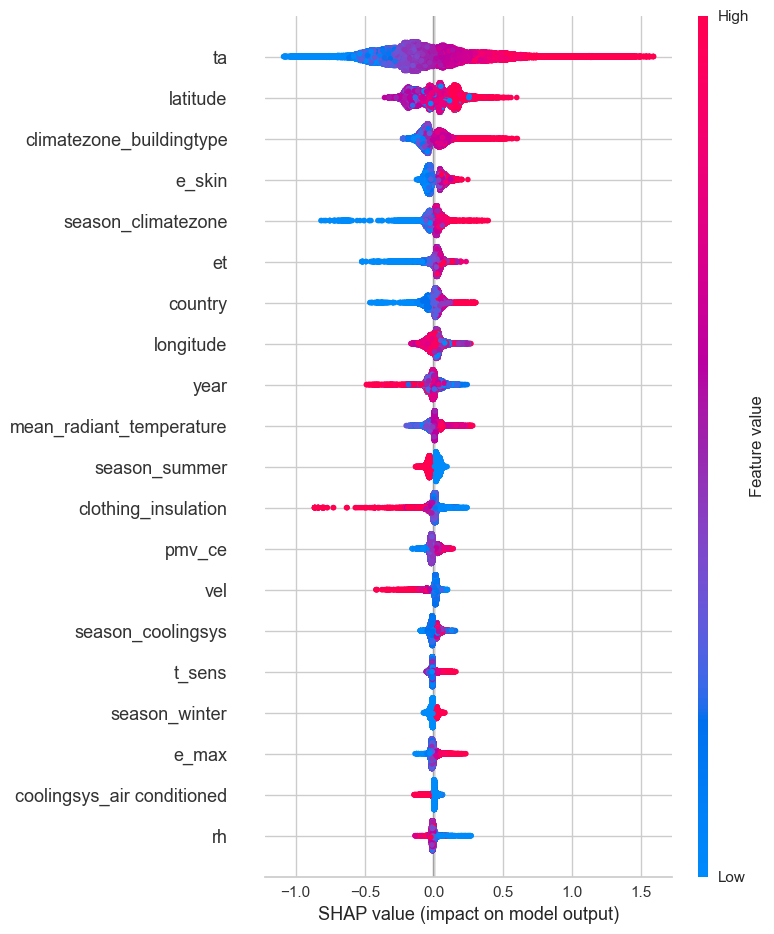
\includegraphics[width=0.75\linewidth]{figures/shapley_pycaret.png}
    \caption{ShaplEY values of the overall thermal comfort datasets fitted to a 10-fold LightGBM model (Full variable definitions provided in Appendix)}
    \label{fig:lgb-featimp}
\end{figure}

% interpreting the implications
Therefore, when looking at the figure again, aside from noticing that the top 20 features predominantly consist of environmental parameters and derived physiological parameters that drives the prediction of thermal comfort, it is worth pointing out that some of the compounded categorical features such as the \textit{climate zone} and \textit{cooling system} making it to the list above \textit{air velocity} and \textit{relative humidity} points to an interesting gap in existing research paradigm where there is a stronger belief that future data collection should be directed to temporal changes of transient environmental/physiological conditions rather than season/system/climate-driven information. Similarly, highly-ranked latitude and longitude suggest that spatial context may capture localized micro-climatic and building-specific effects, pointing to interesting room for further research as they are demonstrating strong predictive power to thermal sensation.

The SHAP value analysis in Figure~\ref{fig:lgb-featimp} provides crucial insights into both feature importance and underlying data quality issues that motivate our physics-informed approach. The prominence of compound categorical features (climate zone, cooling system) above traditional physical variables (air velocity, relative humidity) suggests that spatial and system-level effects are capturing variance not adequately represented by local environmental measurements alone. This finding indicates potential measurement gaps or inconsistencies in the underlying datasets—precisely the type of data quality issues that our PINN framework is designed to address.

Notably, the high ranking of latitude and longitude demonstrates that geographic location serves as a proxy for unmeasured environmental factors, building characteristics, or cultural differences in thermal perception. While this geographic signal provides predictive power, it also highlights the limitations of treating thermal comfort as a purely local environmental phenomenon. Our PINN's energy balance constraints help interpret these geographic effects by ensuring that any learned spatial patterns must remain consistent with fundamental physiological principles, preventing the model from learning spurious geographic correlations that contradict known thermophysiology.

Furthermore, the presence of derived physiological parameters ($e_{skin}$) among the top features validates our approach of incorporating computed physiological variables, while the physics constraints ensure these derived features maintain physiological plausibility despite potential uncertainties in their calculation. This analysis demonstrates how feature importance patterns can reveal data quality challenges that traditional ML approaches cannot address but which physics-informed constraints can effectively regularize.

\subsection{Model Performance}

We ended up comparing outputs from purely neural net models (Vanilla, taking only PMV inputs as its modeling inputs), physiological-MSE-only models (`Physio\_'), physiological-MSE-and physiological constraints models (`Complex\_') as well as heat balance on top of all other custom conditions (`HB\_') as expressed in various prefix and suffix of model used (Gagge/JOS-3) to generate physiological variables. The model performance is presented in Table~\ref{tab:models}. All experiments were conducted on MacBook Pro laptops (M1 Max and M3 Max processors) with random seeds enabled for reproducibility. No discernible performance differences were observed between the two hardware configurations. Training times (TT) are reported in seconds and reflect the computational efficiency of each model variant under identical conditions. Python implementations used the latest supported versions of PyCaret and PyTorch at the time of experimentation.

\begin{table}[htbp]
\centering
\begin{tabular}{l|c|c|c|c|c}
\hline
Model Names & MSE & RMSE & MAPE & MAE & TT (Sec) \\
\hline\hline
Vanilla  & \textbf{1.183685} & \textbf{1.087973} & $20.478$ & \textbf{0.820271} & $67.15$\\
Physio\_Gagge  & $1.221763$ & $1.105334$ & $23.445$ & $0.831138$ & $68.46$ \\
Physio\_JOS3  & $1.281547$ & $1.132055$ & $15.028$ & $0.852872$  & $69.61$\\
Complex\_Gagge  & $1.243027$ & $1.114911$ & $14.482$ & $0.843190$ & $74.60$\\
Complex\_JOS3  & $2.128490$ & $1.458935$ & \textbf{3.393} & $1.176164$ & \textbf{34.43}\\
HB\_Gagge  & $1.459579$ & $1.208130$ & $19.910$ & $0.918638$ & $46.05$\\
HB\_JOS3  & $1.653950$ & $1.286060$ & $14.381$ & $1.030247$ & $46.52$\\\hline
\end{tabular}
\caption{Performance Metrics of Models Tested and Computational Time}
\label{tab:models}
\end{table}

The overall performance metric alone does not tell us enough about how the model performances across the various ranges of $TSV$ from the underlying data, hence we further examined the RMSE and MAPE of seven NN models against their baseline, i.e. the most conventionally accepted metric, $PMV_{CE}$ values as was calculated in the dataset (Figure~\ref{fig:relative-pmv}). 
\begin{figure}[htbp]
    \centering
    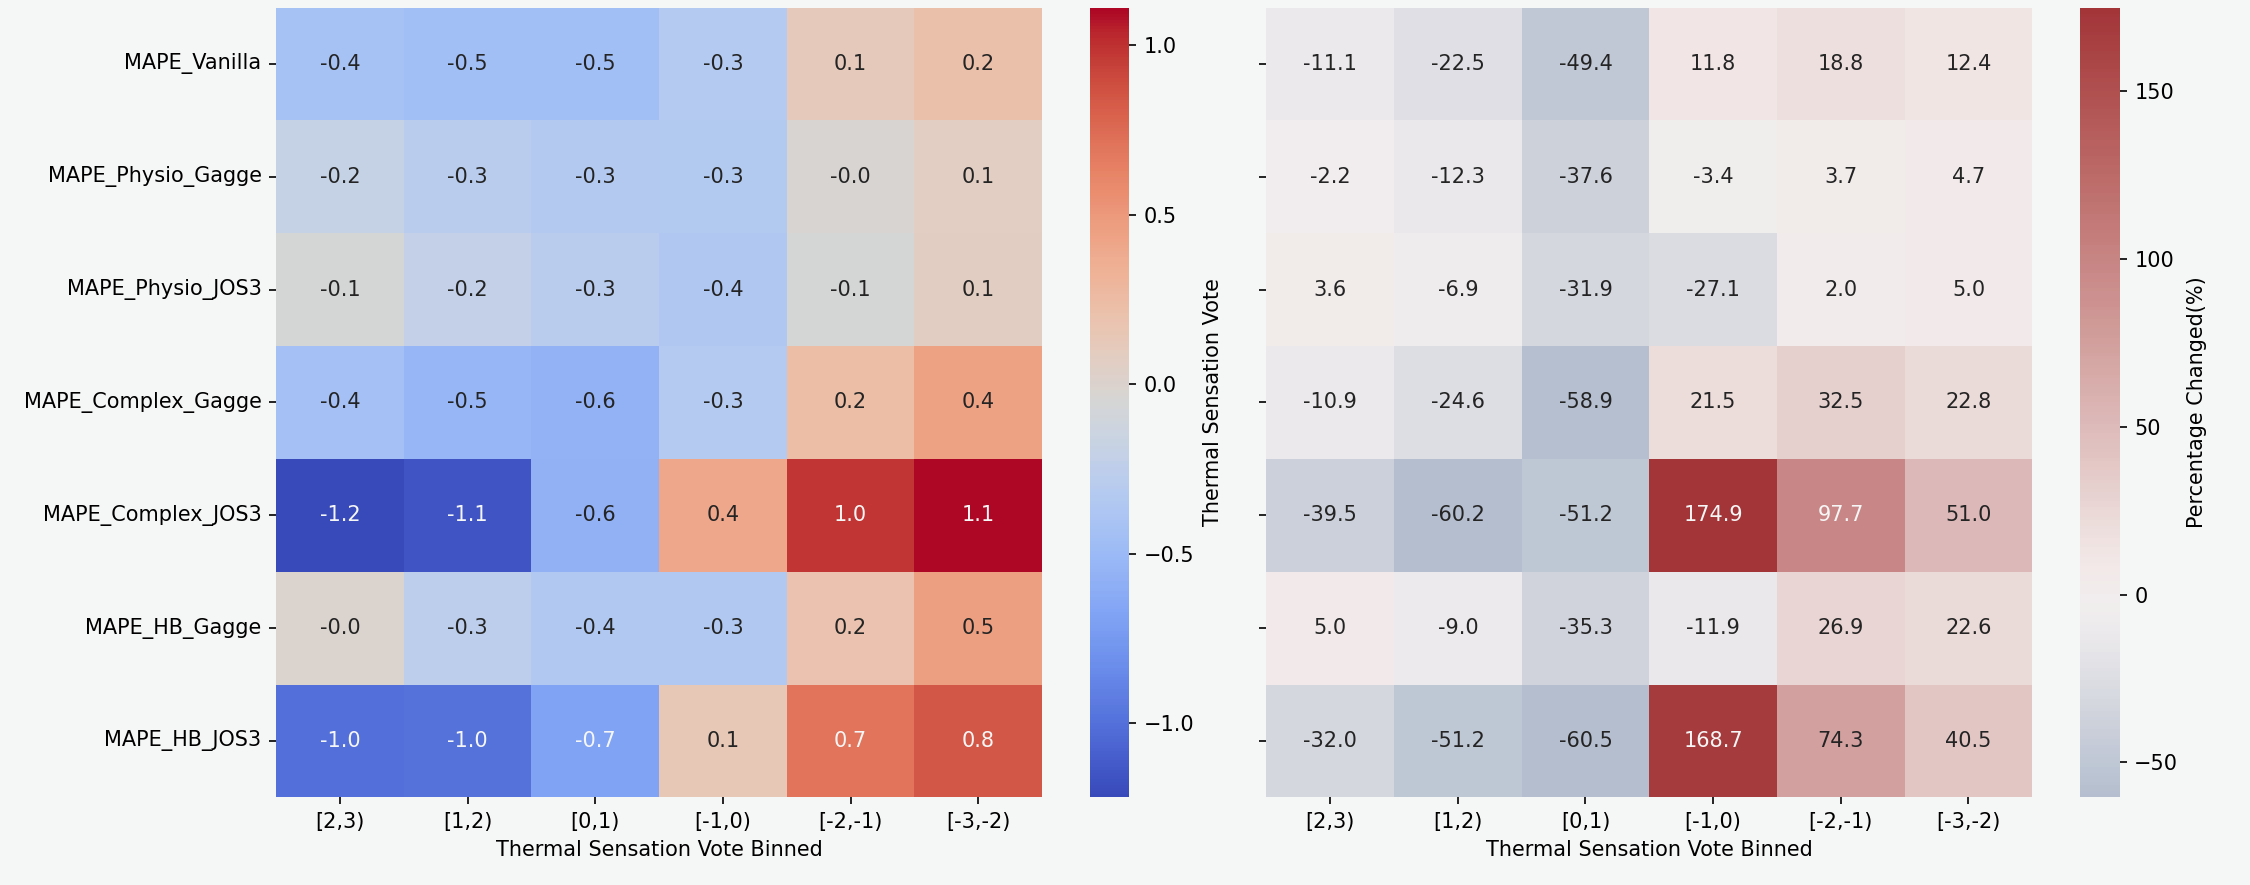
\includegraphics[width=\linewidth]{figures/RMSE_MAPE (1).png}
    \caption{Alternative model prediction performance relative to PMV as baseline (left: RMSE, right: MAPE).}
    \label{fig:relative-pmv}
\end{figure}

As explained in Section~\ref{subsubsec:metrics}, sign-win/loss and range-win/loss-based metrics are introduced to evaluate the models in more discrete and practical approach. SWR and SLR as defined in Equations~\eqref{eq:swr}--\eqref{eq:slr} are calculated to confirm how well the models are capturing the direction of thermal sensation, as shown in Figure~\ref{fig:sign-winloss}, which demonstrated that the Complex\_ and HB\_ models have higher SWR than Vanilla NN and baseline when the $TSV$ is over 0. For the IWR result as shown in Figure~\ref{fig:in-range-sense}, we could clearly see that most of our models outperform the $PMV_{CE}$ model in the moderate thermal sensation range [-1,1].

The superior performance of our PINN models in the moderate thermal sensation range [-1,1] (Figure~\ref{fig:in-range-sense}) addresses a critical need in practical thermal comfort applications. This range represents the zone where most building occupants spend the majority of their time and where HVAC control decisions have the greatest impact on energy efficiency and occupant satisfaction. While concerns about model performance in extreme ranges are noted, our results demonstrate that physics constraints specifically improve prediction accuracy where it matters most for building operations.

The improved IWR performance in the [-1,1] range (average 78.06\% for PINN variants vs. 58.9\% for baseline) reflects the physics constraints' ability to regularize learning toward physiologically consistent patterns. In moderate thermal conditions, human thermoregulation operates within well-established physiological bounds that our energy balance constraints can effectively enforce. This contrasts with extreme thermal conditions, where individual physiological responses become more variable and harder to constrain using steady-state energy balance assumptions.

Importantly, the performance gains in the comfort-critical range validate our core hypothesis: physics-informed constraints provide the greatest benefit where physiological relationships are most predictable and where accurate predictions have the highest practical value. For building control applications, accurate prediction in the [-1,1] range enables proactive HVAC adjustments that maintain comfort while optimizing energy consumption, representing a significant improvement over traditional approaches that struggle with subtle comfort distinctions in this critical operational zone.

\begin{figure}[htbp]
    \centering
    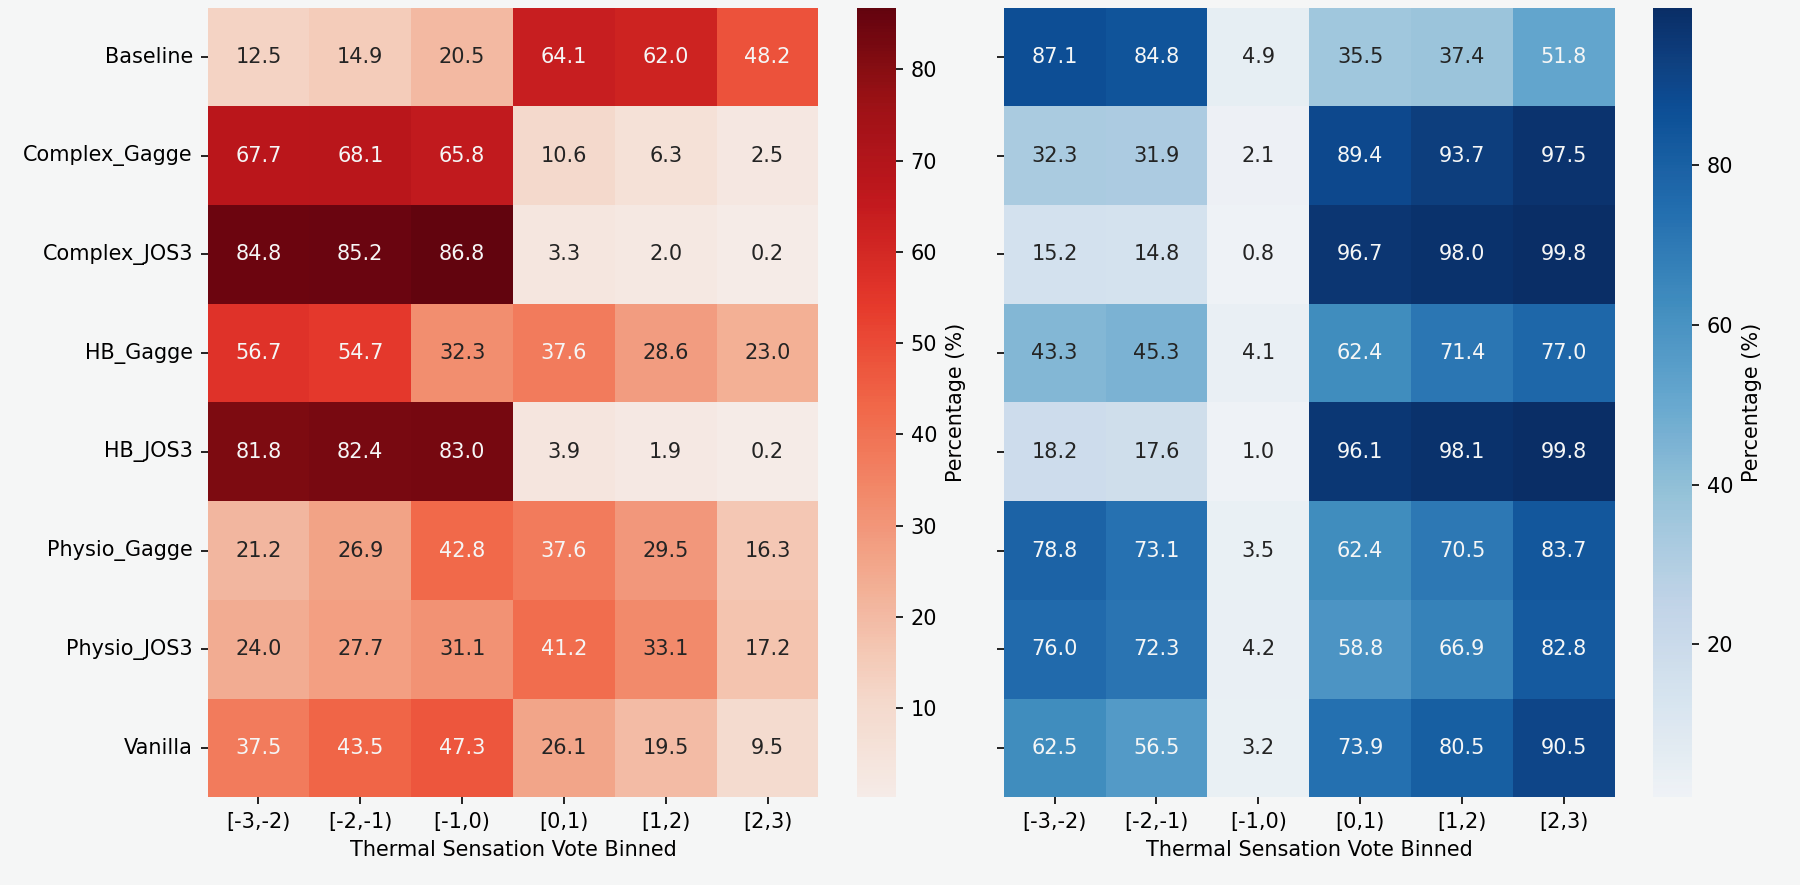
\includegraphics[width=0.95\linewidth]{figures/SignWL (1).png}
    \caption{Heat map of model SLR (left) /SWR (right) across $TSV$ intervals.}
    \label{fig:sign-winloss}
\end{figure}
\begin{figure}[htbp]
    \centering
    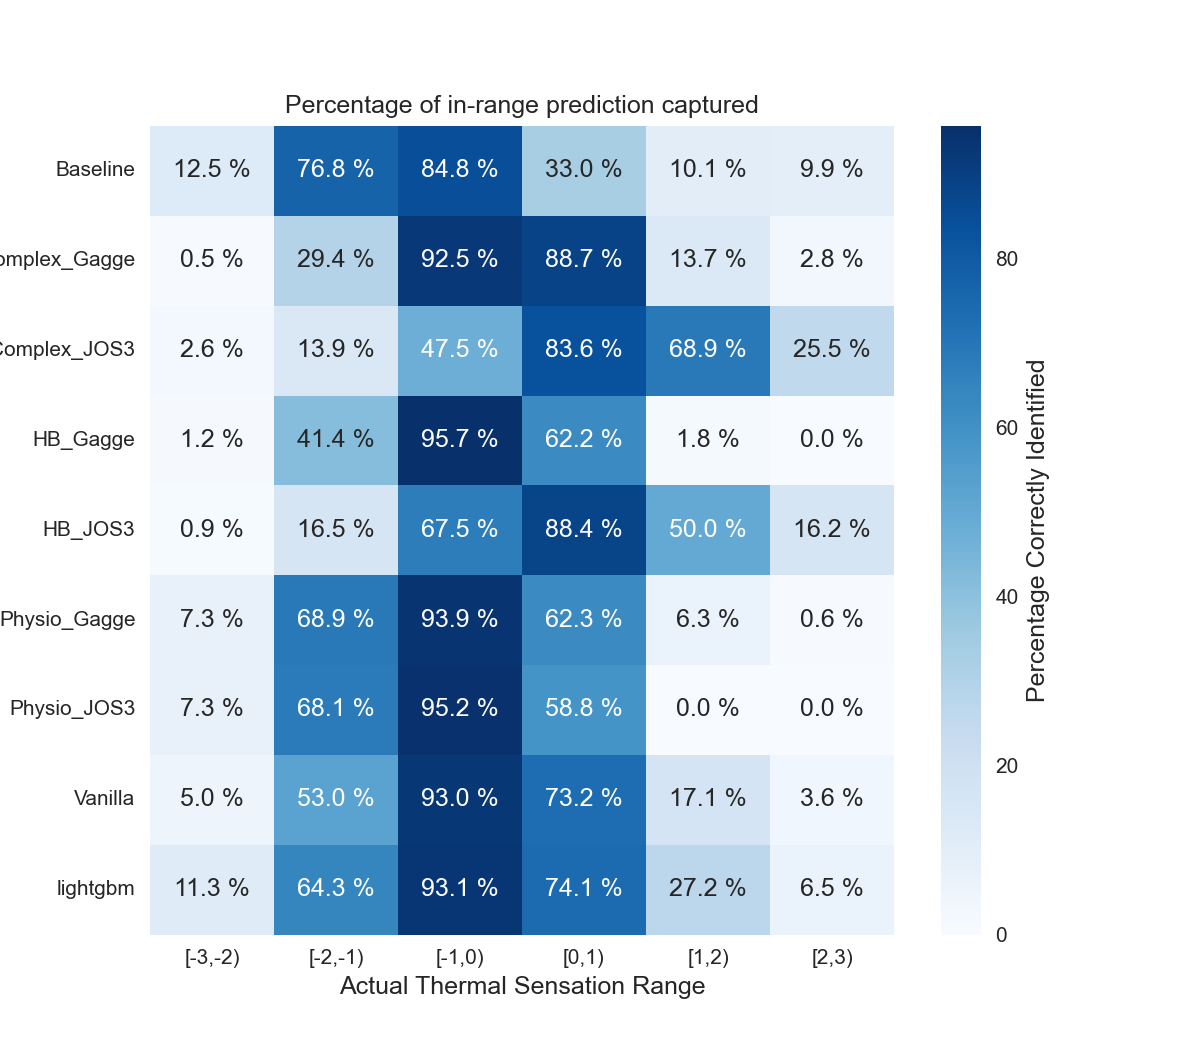
\includegraphics[width=0.75\linewidth]{figures/InRangeSense.png}
    \caption{IWR distribution (rate of prediction within exact matching interval) }
    \label{fig:in-range-sense}
\end{figure}

On top of that, we also want to explicitly highlight the PINN framework's capability by showing its improvement upon $PMV_{CE}$. We did this across all models we fitted, including the regressor model LightGBM. Here we see most of the PINN models showed clear improvements upon $PMV_{CE}$ in term of in-range wins count, except for a few less-populated ranges such as [-2,-1] (Figure~\ref{fig:enter-label}), which is also supported by comparing directly on the FER  performances of models in Figure~\ref{fig:far-off}. 

\begin{figure}[htbp]
    \centering
    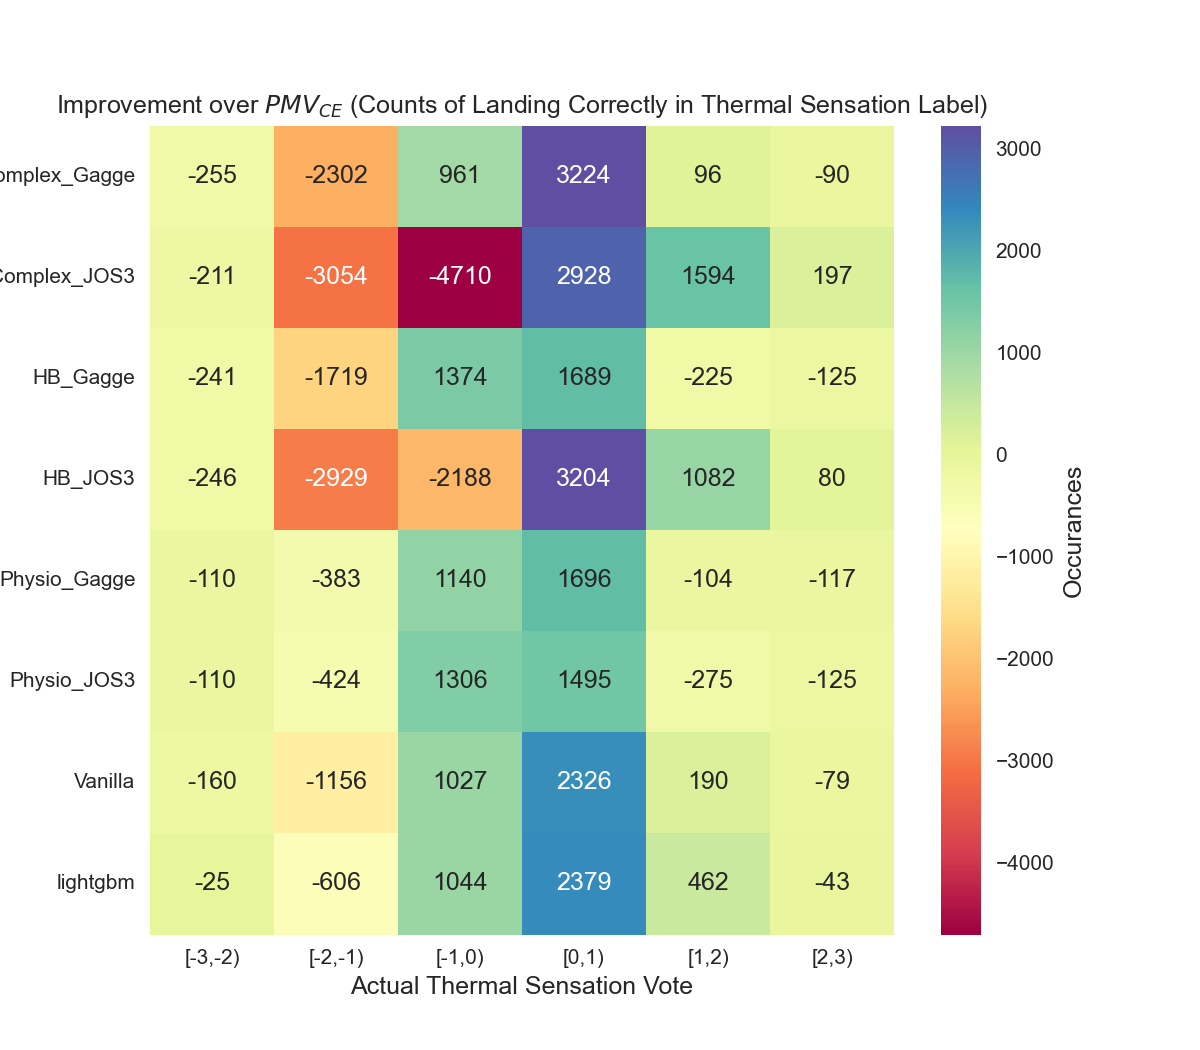
\includegraphics[width=0.75\linewidth]{figures/Improve_Count_PMV.png}
    \caption{In-range wins improvement upon $PMV_{CE}$: Purple-green shows improvement and red shows deterioration.}
    \label{fig:enter-label}
\end{figure}
\begin{figure}[htbp]
    \centering
    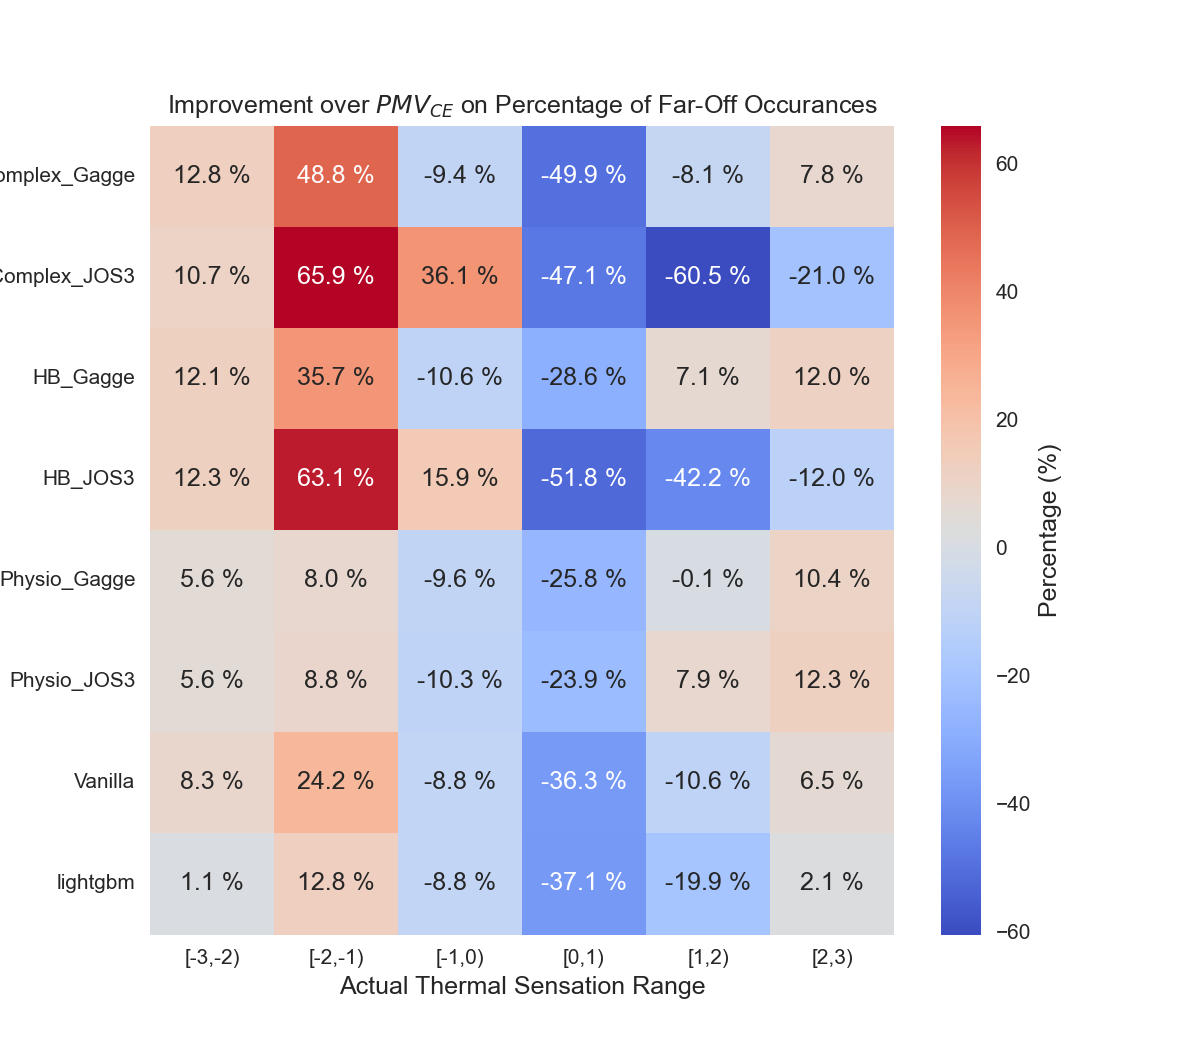
\includegraphics[width=0.75\linewidth]{figures/FOff_Mods_Perc.png}
    \caption{FER (rate of prediction falling outside matching and adjacent intervals) distribution compared to $PMV_{CE}$ }
    \label{fig:far-off}
\end{figure}

\subsection{Analysis of PINN Intermediate Outputs} 

\subsubsection{Distribution across various constraint boundaries}
During our simulation process, we also output $T_{core}$ and  $T_{skin}$ as intermediate outputs for us to better interpret how the modeling process happens, and the additional custom loss function put constraints on the model fitting process.

To better examine our intermediate outputs, we first examined how they are distributed across various constraints that we assigned. For the previous part of the paper, we were setting the constraints for $T_{core}$ to be between 35 and 38 \textdegree{}C and $T_{skin}$ to be between 30 and 35 \textdegree{}C, both commonly acknowledged in the existing literature. However, comparing the actual distribution of calculated $T_{core}$ and  $T_{skin}$, only the $T_{skin}$ limitation applies, given that the actual $T_{core}$ strictly sits within the range of 36.5 to 37.5 \textdegree{}C. We hence proceeded to examine these temperature distribution across three additional ranges that were previously identified by Kingma et al.\cite{kingmaClassicThermoneutralZone2014} on the thermalneutral zones, pointing to potentially either loosening up the $T_{skin}$ to between 30.5 and 36.5 \textdegree{}C, or for comfort consideration, between 31.5 and 35.5 \textdegree{}C, or even a narrower range for very strict thermal comfort between 32.5 and 33.5 \textdegree{}C. We therefore reran the same model architecture, but with these different constraints to assess how well are the custom loss functions performing against each other, as shown in Supplementary Material Figure S1.

Interestingly enough, despite that the constraint was only set upon $T_{skin}$, and the $T_{core}$ constraint remained unchanged between 30 and 35 \textdegree{}C, the resulting $T_{core}$ predicted from the models also saw a trend of being squeezed towards its distribution mean at 36.8 \textdegree{}C in Figure~\ref{fig:squeeze-core}.

\begin{figure}[htbp]
    \centering
    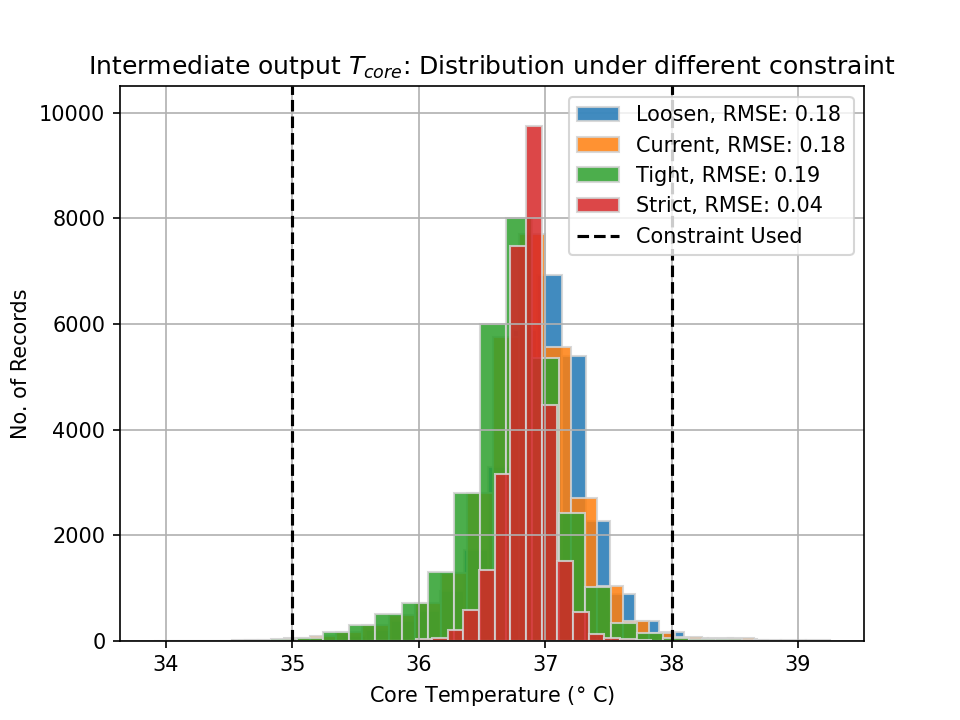
\includegraphics[width=0.65\linewidth]{figures/Squeezed.png}
    \caption{Examining the effect of shrinking skin temperature constraints: effect on core temperature predictions}
    \label{fig:squeeze-core}
\end{figure}

% t_s and Tcr, Tsk error correlation
\subsubsection{Correlation between thermal sensation and intermediate outputs}

To further investigate how the intermediate outputs interact with the $TSV$ predictions, the Pearson correlations of the absolute error of $TSV$ prediction and predicted physiology variables are calculated. (Figure~\ref{fig:error-corr})  HB\_Gagge model (MSE + range penalties on $T_{core}/T_{skin}/w$ + heat balance, using Gagge targets) exhibits a significantly more balanced and positive correlation regarding both variables across different bins compared to other models using Gagge targets, which indicates that the thermodynamic constraint enhances the contribution of intermediate variables to the prediction of thermal sensation.

\begin{figure}[htbp]
    \centering
    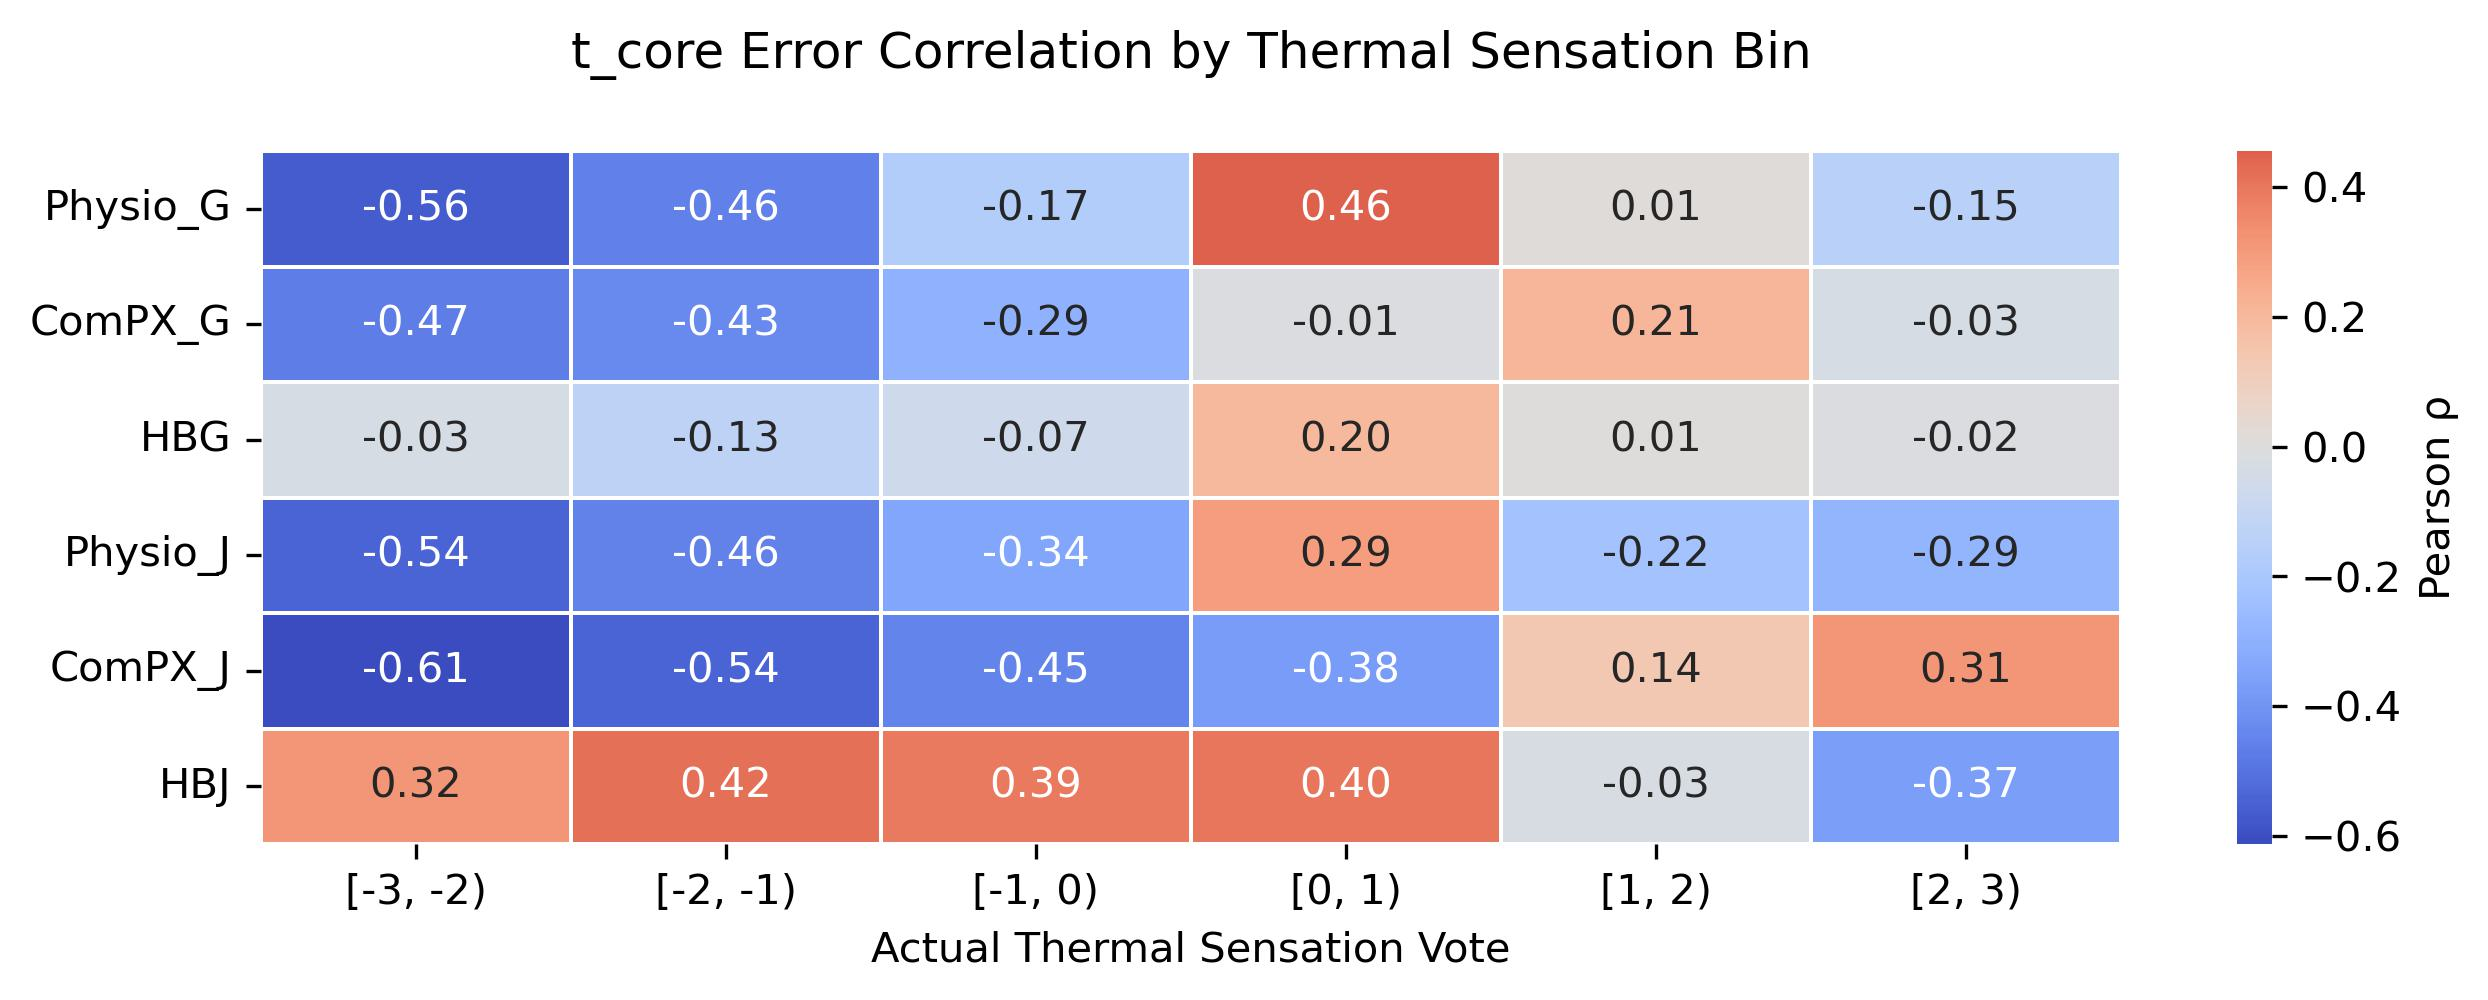
\includegraphics[width=\linewidth]{figures/t_core_ordered_bin_correlations_2.jpg}
    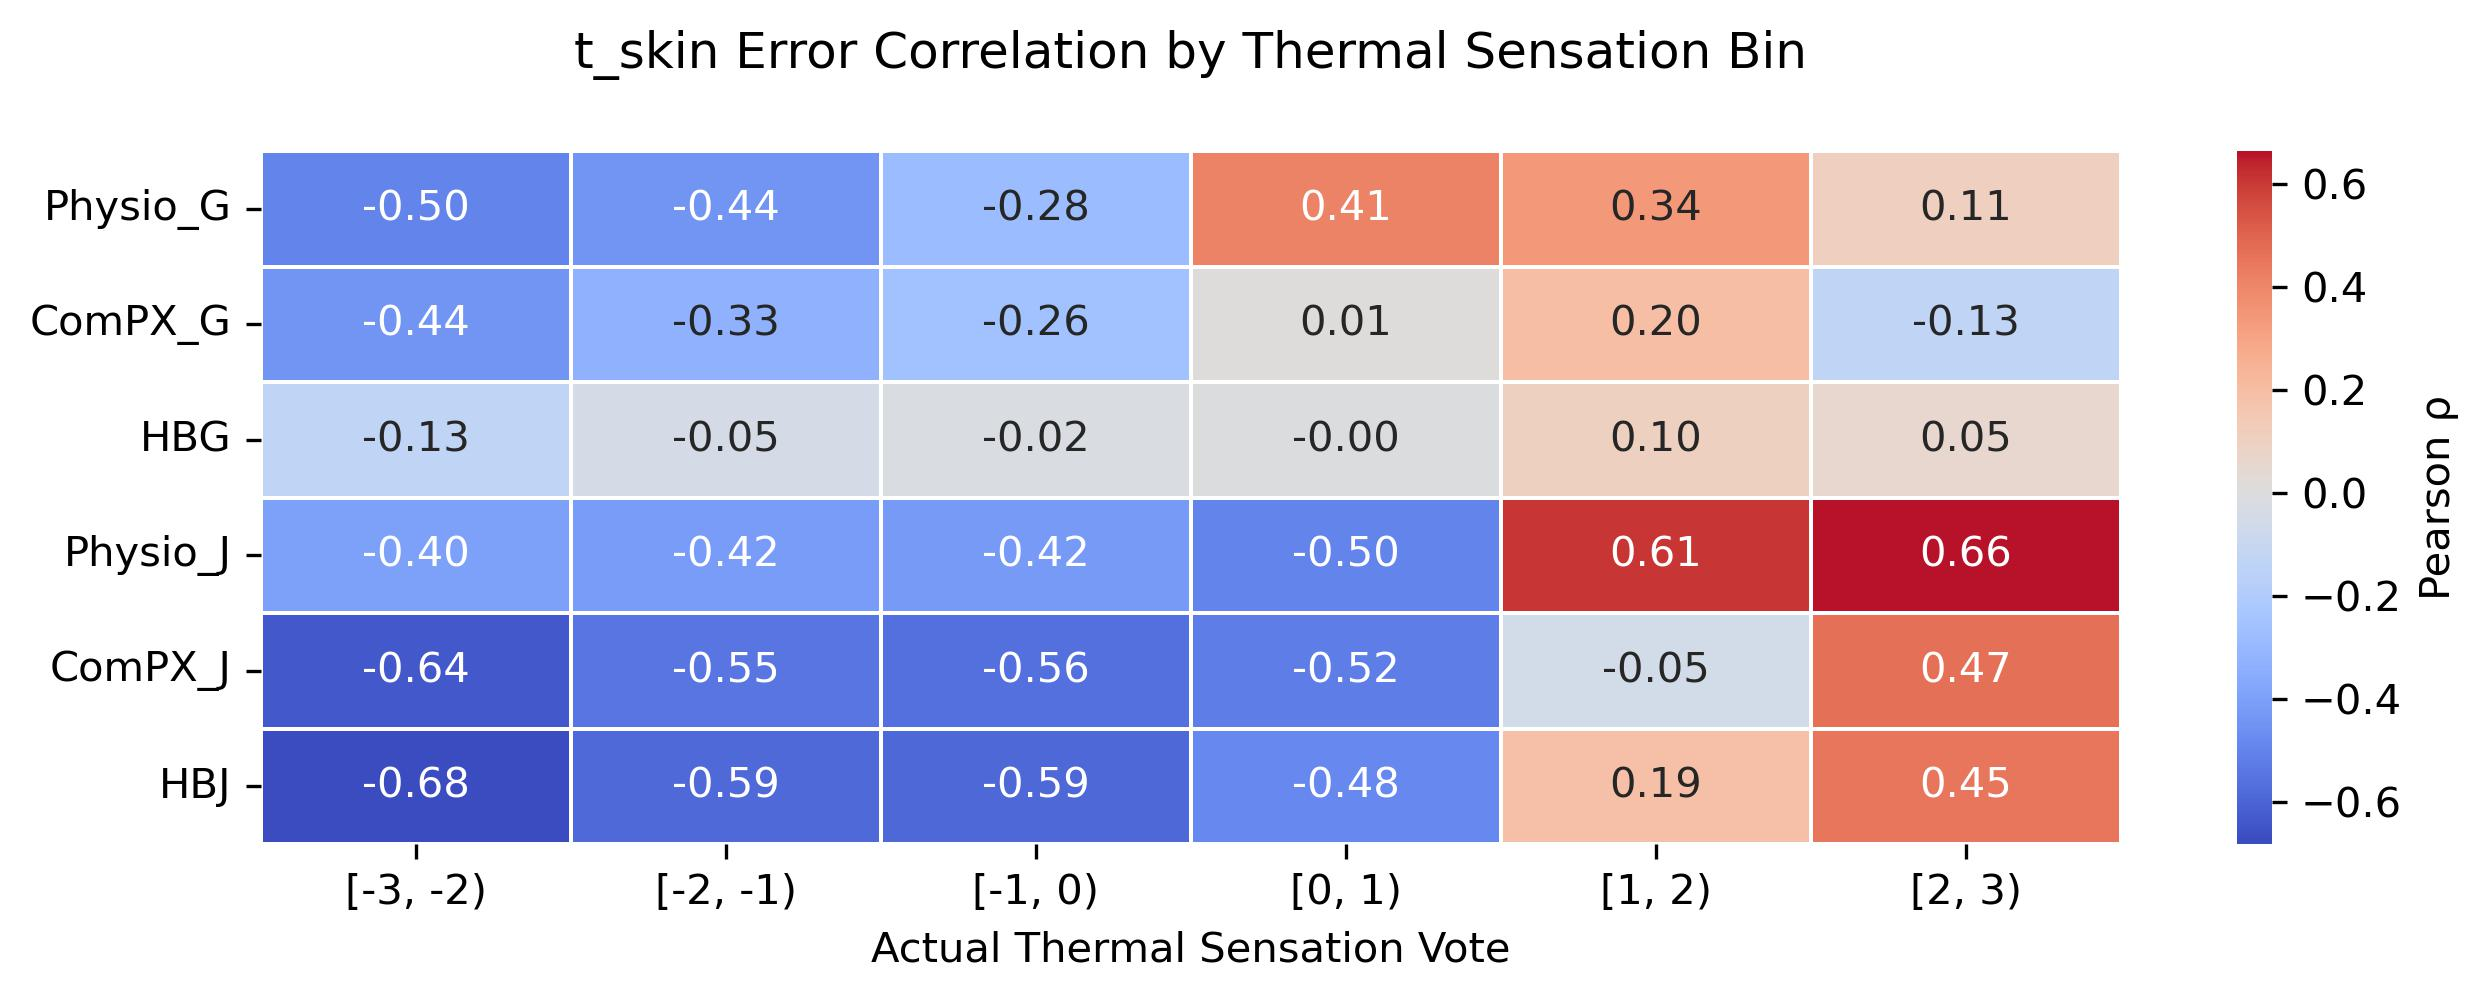
\includegraphics[width=\linewidth]{figures/t_skin_ordered_bin_correlations_2.jpg}
    \caption{Correlation of Thermal Sensation and $T_{cr}$ (above), $T_{sk}$ (below) error}
    \label{fig:error-corr}
\end{figure}

% Regression model of Thermal Sensation and Tcr, Tsk
The strength of physiological constraint can be further explained by building the numeric relationship between $TSV$ and $T_{core}$, $T_{skin}$. Due to the dominating amount of data with thermal sensation within [-1,1] (over 90\% except Complex\_JOS3 and HB\_JOS3), the pattern revealed from the data group ($TSV_{Mild}$) can be more reliable and different from the rest ($TSV_{Extreme}$).
From the linear regression result of $TSV_{Mild}$ group in Supplementary Material Figure S2, both Physio\_ models exhibit abnormally high $R^2$ score along with an unreasonable negative coefficient for $T_{core}$, indicating that the models might find a "backdoor" of learning a deterministic mathematic correlation of the variables, overlooking the hidden physiological mechanism. In comparison, most Complex\_ and HB\_ models appear to be learning more physically plausible correlation, which is also closer to the ground truth. Similar but weaker pattern can also be detected in the $TSV _{Extreme}$ group. The advantageous performance of HB\_ models suggest that future model design could more explicitly incorporate heat balance constraint to improve interpretability and prediction accuracy especially under scenarios involving various thermal sensations.
